\documentclass{article}

% plain.bst is a numeric style, so natbib must be loaded in numeric mode; the
% template documents this hook.
\PassOptionsToPackage{numbers,compress}{natbib}

% ML4PS 2026 workshop, double-blind reviewing.
\usepackage[dblblindworkshop]{neurips_2026}
\workshoptitle{Machine Learning and the Physical Sciences}

% The submission branch of neurips_2026.sty builds the first-page footer from
% \@noticestring.  We redefine only that macro -- the mechanism the style file
% itself provides.  No style-file edits, no layout changes.
\makeatletter
\renewcommand{\@noticestring}{%
  Submitted to the 9th Workshop on Machine Learning and the Physical Sciences (ML4PS 2026). Do not distribute.%
}
\makeatother

\usepackage[utf8]{inputenc}
\usepackage[T1]{fontenc}
\usepackage{hyperref}
\usepackage{url}
\usepackage{booktabs}
\usepackage{amsfonts}
\usepackage{amsmath}
\usepackage{microtype}
\usepackage{graphicx}
\usepackage{wrapfig}

\newcommand{\qcli}{I_{\mathrm{QCLI}}}
\newcommand{\cci}{I_{\mathrm{CCI}}}
% Figures are supplied as vector PDFs; the extension is left off so that a PDF
% supersedes a PNG of the same basename automatically.
\newcommand{\figboxw}[3]{%
  \IfFileExists{#1.pdf}{\includegraphics[width=#3\textwidth]{#1}}{%
    \IfFileExists{#1.png}{\includegraphics[width=#3\textwidth]{#1}}{%
      \fbox{\parbox[c][#2][c]{0.95#3\textwidth}{\centering figure pending: \texttt{#1}}}}}}
\newcommand{\figbox}[2]{\figboxw{#1}{#2}{1.0}}

\title{IQP Generative Models for Strong Gravitational Lensing Images}

% Double-blind submission: the dblblindworkshop option suppresses the author block.
\author{}

\begin{document}

\maketitle

\begin{abstract}
Instantaneous-quantum-polynomial (IQP) circuits are believed hard to sample
classically~\cite{bremner_2011_classical,bremner_2016_average}, while the expectation values a
maximum-mean-discrepancy (MMD) loss needs stay computable, so such a Born machine trains classically
and deploys on quantum hardware~\cite{recio_2025_train}. A recent correlation--complexity map, two
indices from a dataset's Walsh order spectrum and its multi-information, predicts which datasets suit
them, and DeepLense strong-lensing images sit at the most IQP-compatible position we measured
(18-bit tuples $0.47$, $0.87$; the 10-bit crop pmf we train on $0.47$, $0.43$), above the turbulence
data it was introduced on. Given \emph{learned} latent directions
$\theta = \theta^{0} + \Phi^{\!\top} z$, a 10-qubit machine on lens crops is competitive with, and on
some metrics matches, an RBM and a DCGAN carrying $2$--$39\times$ more parameters at 11
training images, and reconstructs unseen images at correlation $0.9684 \pm 0.0004$. Three caveats
bound it. The reference protocol's fixed latent block yields only noise, a structure-matched
permutation null still scores $\qcli = 0.42$, and the DCGAN leads at $100$ images, as the reference
paper predicts. Everything is exact classical simulation at $n = 10$ qubits over five seeds, so we
claim no quantum advantage.
\end{abstract}

\section{Introduction}
\label{sec:intro}

IQP circuits are commuting-gate circuits whose output distribution is the squared Walsh--Hadamard
transform of a phase function. Exact classical sampling from them would collapse the polynomial
hierarchy~\cite{bremner_2011_classical} and the hardness is conjectured to survive approximate
sampling~\cite{bremner_2016_average}, though sufficient noise restores classical
simulability~\cite{rajakumar_2024_polynomial} and classical algorithms exist for some IQP
instances~\cite{codsi_2025_classically}. The same commuting structure keeps an MMD loss's
expectation values computable, so such a model can be \emph{trained classically and deployed on
quantum hardware}~\cite{recio_2025_train,recio_2025_iqpopt}.

Whether real data sits where that is useful is an empirical question, and a recent
proposal~\cite{liu_2026_correlation} approaches it with two ingredients. (i) A
\emph{correlation--complexity map} placing a dataset on two coordinates, the quantum
correlation-likeness indicator $\qcli$, the Jensen--Shannon divergence between the data's Walsh order
spectrum and the i.i.d.\ binomial baseline $b_k = \binom{n}{k}/2^{n}$, and the classical
correlation--complexity indicator $\cci$, how much of its total correlation the best pairwise tree
misses~\cite{watanabe_1960_information,schneidman_2003_network,chow_1968_approximating}, the
high-$\qcli$, high-$\cci$ corner being where IQP circuits should do well. (ii) A
latent-adaptation protocol (Algorithm~1 of the reference paper, which trains a shared phase core on
one anchor, adapts a fixed block of $50$ Walsh-basis phases in Hamming order sample by sample and
interpolates it to unseen samples), both demonstrated on 2D turbulence
snapshots~\cite{khojasteh_2022_lagrangian} at $n=18$ qubits.

We take both to simulated dark-matter strong-lensing images from
DeepLense~\cite{alexander_2020_deep,alexander_2021_decoding}. Lens crops land at the map's most
IQP-compatible position, a 10-qubit IQP Born machine trained on them is competitive with the paper's
own RBM and DCGAN baselines on both metrics at $2$--$39\times$ fewer parameters at 11 images, and
reaches that level only once the protocol's fixed Walsh latent block is made \emph{learnable}. Appendices~\ref{app:turb}--\ref{app:fig4} take the same tests back to the paper's
own data, where its turbulence result does not reproduce under our pre-registered convention and two
internal claims come out mixed.

\begin{figure}[t]
\centering
\figbox{figures/fig1_compact}{2.3in}
\caption{\textbf{(a)} Correlation--complexity map, datasets filled, i.i.d.-uniform nulls open and
labelled null, permutation nulls as crosses (ours, not in the paper). In the legend lens 18b and 18b
pool are the 18-bit per-image and pooled encodings, lens 10b the 10-bit crop pmf, turb.\ D2 and D2
pooled the paper's turbulence data, MNIST-16 and MNIST-784 MNIST at $4\times4$ and $28\times28$,
Blobs BinaryBlobs. \textbf{(b)} First three unconditional samples per
model, $N{=}100$, no selection, shared $0$--$1$ colour scale.}
\label{fig:map}
\end{figure}

\section{Setup}
\label{sec:setup}

\paragraph{Model.}
We compare the reference protocol against its fixed $50$-phase block trained \emph{jointly} across
images and against our \emph{learned-direction} model, a trainable $\Phi$ of $M$ phase-space
directions, each image a point $z_i$ in $M$ dimensions,
\begin{equation}
\theta_i \;=\; \theta^{0} + \Phi^{\!\top} z_i,
\qquad \theta^{0}\in\mathbb{R}^{1024},\quad
\Phi\in\mathbb{R}^{M\times 1024},\quad z_i \in \mathbb{R}^{M},
\label{eq:affine}
\end{equation}
with $M{=}4$ in Table~\ref{tab:main} and $M \in \{0,2,4,6,8,16\}$ in the Fig.~\ref{fig:gen}(a) sweep,
each row of $\Phi$ $L^2$-normalised to $\sqrt{1024}$, and a relative $L^2$ penalty on $z$ of
$\lambda = 10^{-3} L_{0}$, raised to $0.3 L_{0}$ for $M{=}8$, $L_{0}$ being the data loss at
$\theta^{0}$ and $z = 0$. The objectives are the paper kernel (the multi-bandwidth Gaussian
MMD kernel the reference paper takes from IQPopt~\cite{recio_2025_iqpopt}, whose bandwidth rule we
follow since the paper gives none, App.~\ref{app:arms}), the flat MMD (uniform Walsh weights,
estimable from hardware shots) and exact KL (simulation-only); $z$ is drawn from a fitted
Gaussian or resampled with jitter, and $\theta^{0}$ is warm-started by $1{,}000$ exact-KL steps,
itself simulation-only.

\paragraph{Baselines and metrics.}
The baselines are a restricted Boltzmann machine (RBM; 10 visible and 1{,}000 hidden units,
persistent contrastive divergence with one Gibbs
step~\cite{hinton_2002_training,tieleman_2008_training}) and a deep convolutional generative
adversarial network (DCGAN)~\cite{radford_2015_unsupervised}, sized in Table~\ref{tab:main}, both
early-stopped on $200$ validation images disjoint from the held-out set ($160$k or $80$k steps for
the RBM, $5$k to $30$k for the DCGAN) while the IQP arms run a fixed $4{,}000$, which can only favour
them. We keep the reference paper's two metrics, the Jensen--Shannon divergence between
intensity histograms (PDF--JS) and Conv2D-MMD$^2$, a biased V-statistic in a fixed random
convolutional encoder's feature space~\cite{gretton_2012_kernel}, and add a held-out projection
correlation. PDF--JS uses $50$ bins fixed on $[0,1]$ and the Conv2D-MMD$^2$ scale and bandwidth come
from the held-out set alone, so neither metric moves with the arm scored, and the floor is $20$ draws
of $200$ against $200$ disjoint validation images (App.~\ref{app:arms}). Every IQP arm and the RBM
share the
flux scalar $S$ while the DCGAN learns its own, so raw Conv2D-MMD$^2$ is partly a brightness
comparison and we add a flux-aligned variant, flagged as post-hoc, rescaling every image to the
held-out mean total intensity. Every arm generates 200 images scored against the same 200
held-out images at $N \in \{11,100\}$, every number a mean $\pm$ sample sd over five seeds, and the
projection optimises $z$ from eight restarts (App.~\ref{app:arms}).

\paragraph{Departures from the reference setup.}
Six choices differ from the reference paper, each following from the data. Its snapshots interpolate
to unseen times, whereas the DeepLense \texttt{Model~II} images we
use~\cite{alexander_2020_deep,alexander_2023_domain,ml4sci_deeplense} are static in three classes, so
we generate unconditionally from the latent prior. It encodes a sample as 18-bit
$(x,y,\mathrm{intensity})$ tuples, whereas we centroid-align each $64\times64$ image and read its
central $32\times32$ crop, $99.4\%$ of the light, as one probability mass function (pmf) over
$1{,}024$ cells at $n=10$ (App.~\ref{app:pipe}), a raw intensity axis carrying barely one bit. Its
anchor-and-adapt protocol fixes the latent block, whereas we learn $\Phi$ and train the $N$ images
jointly (Sec.~\ref{sec:whyfail}), and it estimates its MMD from $500$ samples per step where a
$10$-qubit pmf is exact. It holds out times, which static images lack, so we project onto held-out
images. Each generated crop is pasted back into $64\times64$ at the training-set mean total intensity
$S$ ($112.3$ at $N{=}11$, $124.9$ at $N{=}100$; held-out $123.9$) and a training-set offset.

\section{Results}
\label{sec:results}

\subsection{Lens images are the most IQP-compatible dataset on the map}
\label{sec:map}

Table~\ref{tab:map} recomputes the map. Encoded as the reference paper encodes turbulence, lens
images sit far above it in $\qcli$ and inside the corner the map calls IQP-compatible, yet a
permutation null that keeps each image's intensity histogram and destroys spatial structure nearly
matches them, and turbulence behaves the same way, so at this encoding the map largely tracks the
histogram. Only the 10-bit crop pmf we train on separates from its null in both coordinates, so a
favourable position is necessary, not sufficient.

\begin{table}[tb]
\centering
\caption{Correlation--complexity map on our data, each permutation null keeping the value histogram
of the row above, mean $\pm$ sd over five seeds. $K$ is the number of $n$-bit codes per image or
snapshot; the lens 18-bit row sweeps all $4{,}096$ $(k_x,k_y)$ cells of a $64\times64$ image and so
has no sampling noise, while the turbulence row subsamples a larger grid. Both are $K$-dependent, so
a row reads only against its own-$K$ null, and at the paper's own $K = 5\times10^{4}$ the turbulence
$\qcli$ is $0.091 \pm 0.000$ against a null of $0.098 \pm 0.001$.}
\label{tab:map}
\scriptsize
\begin{tabular}{llcc}
\toprule
Dataset and encoding & $K$ & $\qcli$ & $\cci$ \\
\midrule
Lens, 18-bit $(x, y, \mathrm{intensity})$ tuples & $4{,}096$ & $0.4715 \pm 0.0000$ & $0.8677 \pm 0.0000$ \\
\quad permutation null            & $4{,}096$ & $0.4154 \pm 0.0000$ & $0.8783 \pm 0.0001$ \\
Turbulence D2, 18-bit tuples       & $4{,}096$ & $0.0232 \pm 0.0002$ & $0.9285 \pm 0.0008$ \\
\quad permutation null            & $4{,}096$ & $0.0114 \pm 0.0000$ & $0.9371 \pm 0.0009$ \\
\midrule
Lens, 10-bit crop pmf              & exact pmf & $0.4731 \pm 0.0000$ & $0.4313 \pm 0.0000$ \\
\quad permutation null            & exact pmf & $0.1782 \pm 0.0000$ & $0.9634 \pm 0.0004$ \\
\bottomrule
\end{tabular}
\end{table}

\subsection{Why the reference protocol needs learned directions}
\label{sec:whyfail}

Run sequentially on our low-variance latent block, Algorithm~1 produces noise
(Fig.~\ref{fig:map}(b), second row; App.~\ref{app:arms} has the Hamming-ordered variant).
Representability is not the cause, since the full 1{,}024-phase circuit fits a \emph{single} aligned
crop to correlation $0.99997 \pm 0.00001$ under the flat MMD. The protocol is. With the core frozen
on one anchor, the 50 fixed latent coordinates reconstruct every other training image at only
$0.44 \pm 0.04$, fixed Walsh directions cross-fading pixels as an XOR-shift interference pattern
instead of moving lens structure.

\subsection{Learned latent directions generalise}
\label{sec:affine}

Equation~\eqref{eq:affine} repairs this. Freezing $\theta^{0}$ and $\Phi$ and optimising only $z$ on
200 \emph{held-out} images, the best arm at $N{=}100$, flat MMD at $M{=}4$, reaches mean correlation
$0.9684 \pm 0.0004$ against a nearest-training-image reference of $0.970$, the paper kernel reaching
only $0.792 \pm 0.006$ at $N{=}11$ and $0.805 \pm 0.012$ at $N{=}100$. The gain comes from learning
the directions, not the extra parameters, since in the $N{=}20$ sweep of Fig.~\ref{fig:gen}(a) a
trained $\Phi$ beats a random direction on the same latent-free offset ($0.7458 \pm 0.0005$). Useful $M$ also stays small, $M{=}2$ being the best and by far
the most stable ($0.9060 \pm 0.0021$ against $0.8577 \pm 0.0559$ at $M{=}4$), with collapse by
$M{=}8$ ($0.218 \pm 0.121$) once the required $\|z\|$ exceeds the coherence radius.

\begin{figure}[t]
\centering
\figbox{figures/fig2_compact_seeds}{2.0in}
\caption{Different experiments. \textbf{(a)} Controlled latent-width sweep ($N{=}20$), held-out
projection correlation against $M$, mean $\pm$ sd over five model seeds, with its own reference levels
($0.934$ nearest training image, $0.744$ mean training image, $0.746$ a random direction on the
latent-free $M{=}0$ offset); $M{=}8$ and $16$ are best over a learning-rate sweep selected on the
plotted correlation, $M{=}0$ and $M{=}4$ single-rate. \textbf{(b)} Round-3b arms at $N{=}100$,
held-out crops, then $M{=}4$ flat MMD, $M{=}4$ paper kernel and the collapsed $M{=}8$ arm.}
\label{fig:gen}
\end{figure}

\begin{table}[t]
\centering
\caption{Paper-style comparison on lens crops, mean $\pm$ sd over five seeds, PDF--JS in $10^{-3}$
and both MMD$^2$ columns in $10^{-2}$. Lower is better; \textbf{bold} marks a best mean leading the
runner-up by more than both sds, so a column without bold carries no win the seed spread supports.
Params are totals at $N{=}11\,/\,N{=}100$; MMD$^2_{\mathrm{al}}$ is flux-aligned (post-hoc) and the
last row a real-vs-real floor over $20$ draws of $200$ against $200$. App.~\ref{app:arms} gives $^{\dagger}$
and the parameter convention.}
\label{tab:main}
\scriptsize
\setlength{\tabcolsep}{2pt}
\begin{tabular}{lrcccccc}
\toprule
& & \multicolumn{3}{c}{$N = 11$} & \multicolumn{3}{c}{$N = 100$} \\
\cmidrule(lr){3-5}\cmidrule(lr){6-8}
Model & Params & PDF--JS & MMD$^2$ & MMD$^2_{\mathrm{al}}$ & PDF--JS & MMD$^2$ & MMD$^2_{\mathrm{al}}$ \\
\midrule
IQP, reference protocol (Alg.~1)$^{\dagger}$ & 1{,}524 / 5{,}974 & 7.2\,$\pm$\,0.7 & 18.8\,$\pm$\,1 & 22.5\,$\pm$\,2 & 8.4\,$\pm$\,0.4 & 21.8\,$\pm$\,0.6 & 26.6\,$\pm$\,0.7 \\
IQP, fixed basis, joint           & 1{,}524 / 5{,}974 & 1.6\,$\pm$\,0.4 & 12.3\,$\pm$\,0.4 & 12.5\,$\pm$\,1 & 1.0\,$\pm$\,0.1 & 10.2\,$\pm$\,0.8 & 8.5\,$\pm$\,1 \\
IQP, learned dir.\ $M{=}4$ (flat MMD) & 5{,}164 / 5{,}520 & 3.0\,$\pm$\,0.2 & 8.9\,$\pm$\,0.2 & 2.7\,$\pm$\,0.2 & 2.9\,$\pm$\,0.3 & 7.2\,$\pm$\,0.3 & 2.6\,$\pm$\,0.4 \\
IQP, learned dir.\ $M{=}4$ (paper kernel) & 5{,}164 / 5{,}520 & 0.81\,$\pm$\,0.05 & 9.6\,$\pm$\,0.3 & 7.4\,$\pm$\,0.6 & 1.4\,$\pm$\,0.2 & 11.3\,$\pm$\,0.5 & 10.0\,$\pm$\,0.8 \\
RBM~\cite{tieleman_2008_training}  & 11{,}510 / 15{,}960 & 1.7\,$\pm$\,0.8 & 6.5\,$\pm$\,0.8 & 11.1\,$\pm$\,4 & 0.9\,$\pm$\,0.1 & 5.9\,$\pm$\,0.4 & 8.1\,$\pm$\,2 \\
DCGAN~\cite{radford_2015_unsupervised} & 199{,}837   & 1.1\,$\pm$\,0.6 & 5.1\,$\pm$\,2 & 3.9\,$\pm$\,1 & \textbf{0.55}\,$\pm$\,0.12 & \textbf{2.2}\,$\pm$\,0.3 & 2.1\,$\pm$\,0.4 \\
\midrule
\textit{Real-vs-real floor} & n/a & \textit{0.04}\,$\pm$\,0.02 & \textit{0.5}\,$\pm$\,0.3 & \textit{0.4}\,$\pm$\,0.2 & \textit{0.04}\,$\pm$\,0.02 & \textit{0.5}\,$\pm$\,0.3 & \textit{0.4}\,$\pm$\,0.2 \\
\bottomrule
\end{tabular}
\end{table}


\subsection{Paper-style comparison and data scaling}
\label{sec:table}

In Table~\ref{tab:main} the eleven-image regime is where the IQP arms are competitive. The $M{=}4$
paper-kernel arm holds the best mean PDF--JS there and the $M{=}4$ flat-MMD arm the best mean
flux-aligned Conv2D-MMD$^2$ at $2$--$39\times$ fewer parameters, but both leads sit inside one sd of
the baselines, so we read them as matching, not beating. Raw Conv2D-MMD$^2$ runs the other way
at both sizes, both baselines ahead of every IQP arm, an ordering the flux-aligned column partly
reverses. At $N{=}100$ the DCGAN leads all three columns, decisively on PDF--JS and raw
Conv2D-MMD$^2$ and within the $M{=}4$ flat-MMD arm's spread on the flux-aligned one.
That ordering is the reference paper's data-scaling picture, traced across $N$ in
Fig.~\ref{fig:scaling}. Trained inside one class, the same arm holds a projection correlation of
$0.969$--$0.972$ with PDF--JS and Conv2D-MMD$^2$ at the pooled level, each against its own floor
(Table~\ref{tab:classes}).

\section{Discussion and limitations}
\label{sec:disc}

Nothing here is evidence of quantum advantage, since every circuit is simulated exactly at $n=10$
qubits and the hardness results describe the class at scale, not our instances. Five seeds are
few, and the DCGAN adds a spread of up to $57\%$ on raw Conv2D-MMD$^2$ and $74\%$ on PDF--JS at one
configuration and seed, cuDNN having no deterministic transposed-convolution kernel. $S$ is imposed
on the IQP arms and the RBM but learned by the DCGAN.

\bibliographystyle{plain}
\bibliography{refs}

\newpage
\appendix

\section{Pipeline}
\label{app:pipe}

Figure~\ref{fig:pipe} summarises the encoding, the latent parameterisation and the evaluation.

\begin{figure}[tb]
\centering
\figboxw{figures/fig_pipeline_v2_c}{3.6in}{0.66}
\caption{Pipeline. \textbf{(a)} A held-out $64\times64$ image, white cross at its intensity centroid
and dashed box the $32\times32$ crop window. \textbf{(b)} The aligned crop read as a pmf over
$1{,}024$ cells, the example pixel $(k_x,k_y) = (12,20)$, the integer form of $(x,y)$, carrying code
$404 = 0110010100_2$ with bit $j$ addressing qubit $j$. \textbf{(c)} The first two learned latent
coordinates of the $100$ training images at $M = 4$. \textbf{(d)} The IQP circuit, an H layer, one
diagonal phase $\exp(i\sum_s \theta_s Z_s)$ over all $1{,}024$ subsets $s$, a second H layer and
measurement.
\textbf{(e)} Exact simulation through $q_\theta = |\mathcal{W}e^{i\theta}|^{2}/2^{n}$, trained jointly
over the $N$ images by MMD (flat or paper kernel) or by KL, the fast Walsh--Hadamard transform (FWHT)
supplying $\mathcal{W}$ and the dashed arrow updating $\theta^{0}$, $\Phi$ and $z$. \textbf{(f)} A
trained $q(x,y)$ scaled by $S$ and pasted at a sampled offset. \textbf{(g)} The intensity PDF of real
against IQP samples (PDF--JS $0.0029$), Conv2D-MMD$^2$ at $N{=}100$ (IQP $0.072$, RBM $0.059$, DCGAN
$0.022$) and projection correlations over $200$ held-out images (mean $0.968$). The bottom row
contrasts a reference-protocol sample with an $M{=}4$ sample from this work.}
\label{fig:pipe}
\end{figure}

\section{Replication of the reference paper's turbulence experiment}
\label{app:turb}

We attempted a direct replication on the reference paper's own dataset (2D cylinder-wake turbulence
D2~\cite{khojasteh_2022_lagrangian}, $n=18$ qubits, 11 anchor snapshots) over five seeds. Under our
pre-registered convention the result is \textbf{not reproduced}, since in the 11-snapshot regime the
RBM (PDF--JS $0.217 \pm 0.007$) and a 1.2M-parameter DCGAN ($0.045 \pm 0.062$) beat our 31k-parameter
IQP ($0.272 \pm 0.004$) on \emph{both} metrics. Two findings qualify this. Under a last-write-wins
aggregation convention, never specified in the paper, our IQP's PDF--JS values land close to the
published ones ($0.0324 \pm 0.0011$ and $0.0473 \pm 0.0005$ against $0.0238$ and $0.0221$, with
Conv2D-MMD$^2$ $0.711 \pm 0.012$ and $0.738 \pm 0.017$), but the RBM still wins. Conv2D-MMD$^2$ is
also saturated, ground truth shuffled in pixel space already scoring $0.7045 \pm 0.0095$, below every
model in the paper's Table~2 ($0.90$--$1.47$), and unseen-time synthesis is solvable by linear
interpolation ($0.9998$, deterministic). Our anchor-fit level ($0.651 \pm 0.010$
sampled, $0.739 \pm 0.010$ exact for the 31k arm) traces to stage~1 freezing the latent block
($-0.114 \pm 0.021$) and to a $0.892$ model-family ceiling that carries no seed, nothing in that fit
consuming the random stream, rather than to our implementation; the $5\times10^{4}$-sample pmf, which
a single seed made look like a second cause, costs nothing measurable over five
($-0.001 \pm 0.022$), and stage~2 adds $0.000 \pm 0.000$.

\section{Support mismatch (reference paper Fig.~3)}
\label{app:fig3}

\begin{figure}[tb]
\centering
\begin{minipage}[t]{0.31\textwidth}\centering
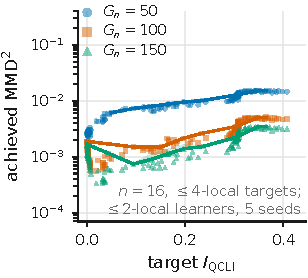
\includegraphics[width=\linewidth]{figures/figA_fig3_c_seeds}
\end{minipage}\hfill
\begin{minipage}[t]{0.31\textwidth}\centering
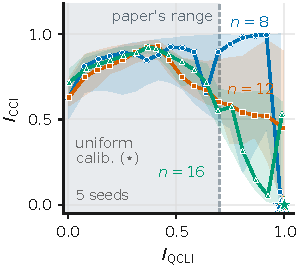
\includegraphics[width=\linewidth]{figures/figA_fig4_c_seeds}
\end{minipage}
\caption{\textbf{(a)} Support-mismatch study at $n=16$, with $140$ target circuits ($\leq 4$-local)
spanning exact $\qcli \in [0, 0.408]$ fitted by $\leq 2$-local learners of $G_n = 50$, $100$ and
$150$ requested gates, $G_n$ being the learner's gate count, the last capped at the $136$ generators
a $\leq 2$-local circuit has at $n = 16$ (exact MMD, Adam, $5{,}000$ steps, five learner seeds). More gates lower the whole envelope (claim (b),
reproduced), while within the reachable range the achieved MMD$^2$ \emph{rises} with target $\qcli$,
the opposite of claim (a). \textbf{(b)} Circuits optimised to maximise $\qcli$ only, $n = 8, 12, 16$,
five seeds and 2 gain settings per $n$, $3{,}333$ steps each and about $33{,}000$ logged points per $n$.
$\cci$ never enters the objective.}
\label{fig:appcd}
\end{figure}

The reference paper's Fig.~3 claims (a) that the upper envelope of achievable MMD falls as the
target's $\qcli$ rises, because the support-induced floor shrinks, and (b) that the envelope drops
overall as the learner gets more gates (Fig.~\ref{fig:appcd}(a)). Claim (b) reproduces, the median
achieved MMD$^2$ falling $9.58\times10^{-3} \to 2.15\times10^{-3} \to 1.44\times10^{-3}$ across the
three learners with a seed spread of at most $2\times10^{-5}$. Claim (a) runs the other way inside
the range we can reach, the achieved MMD$^2$ \emph{rising} as the target's exact $\qcli$ goes from
$0$ to $0.41$ (Spearman $\rho = +0.979 \pm 0.001 / +0.901 \pm 0.001 / +0.809 \pm 0.004$), a trend
that also holds for a control trained on exact pmfs. The paper's premise still holds mechanistically
($\rho \le -0.98$ for the exact-pmf form of the Proposition~II.2 floor proxy and $\le -0.92$ for its
$10^{4}$-sample form), but the achieved MMD is dominated by trainability rather than support
mismatch. Our target family saturates at exact $\qcli \approx 0.41$, and at $0$--$0.064$ when
estimated from $10^{4}$ samples as the paper does, so the regime claim (a) asserts lies outside what
we could build.

\section{\texorpdfstring{The $\qcli$--$\cci$ ceiling}{The QCLI-CCI ceiling}}
\label{app:fig4}

We also reproduced the experiment in which maximising $\qcli$ alone raises $\cci$ as a by-product
(Fig.~\ref{fig:appcd}(b)). The coupling reproduces at low $\qcli$ (pooled Spearman
$\rho = +0.79/+0.79/+0.90$ for $n=8/12/16$ restricted to $\qcli \leq 0.3$, and
$+0.92 \pm 0.10 / +0.91 \pm 0.04 / +0.96 \pm 0.01$ seed by seed) but reverses above
$\qcli \approx 0.38$ at all three sizes once five seeds are pooled (global
$\rho = +0.08, -0.57, -0.64$), the per-seed global $\rho$ itself seed-dependent at the two smaller
sizes ($+0.25 \pm 0.92$ and $-0.52 \pm 0.36$) because whether a trajectory reaches the ceiling inside
$3{,}333$ steps is a property of the seed. The reversal is forced by the definitions, the exactly
uniform distribution maximising $\qcli$ ($0.982/0.998/0.9999$) with $\cci = 0$. The reference paper's
figure stops below $\qcli \approx 0.7$, so a high $\qcli$ need not indicate exploitable structure and
can simply indicate proximity to uniform.

\section{Additional arms}
\label{app:arms}

\begin{figure}[tb]
\centering
\figboxw{figures/figA_scaling_seeds}{2.1in}{0.40}
\caption{Conv2D-MMD$^2$ against training-set size, mean $\pm$ sd over five seeds, raw as solid lines
and flux-aligned as dashed with open markers, over the real-vs-real floor band. Seeds vary the model
only, the training subsets being nested prefixes of one draw.}
\label{fig:scaling}
\end{figure}

\paragraph{Data scaling.} At $N \in \{10,30,50,70,90,100\}$ the learned-direction IQP arm is flat for
$N \geq 30$ (raw Conv2D-MMD$^2$ $0.068$--$0.072$) and so is the RBM ($0.055$--$0.067$), while the
DCGAN leads already at $N{=}10$ ($0.046 \pm 0.017$ against $0.095 \pm 0.002$) and falls a further
$2\times$ by $N{=}100$ ($0.046 \to 0.022$), as Fig.~\ref{fig:scaling} shows. On the flux-aligned column the IQP arm leads
at $N{=}10$ and $N{=}30$ and the DCGAN from $N{=}50$, the two overlapping within a seed sd everywhere
except $N{=}10$ and $N{=}90$.

\paragraph{Exact KL.} KL needs the full simulated distribution and cannot be estimated from hardware
shots, so we keep it out of Table~\ref{tab:main} and record it here at seed~0 only. Its $M{=}2$ arm,
on $3{,}094$ / $3{,}272$ parameters, reaches PDF--JS $0.00172$ at $N{=}11$ and $0.00302$ at
$N{=}100$, raw Conv2D-MMD$^2$ $0.119$ and $0.091$, flux-aligned $0.046$ and $0.075$. The collapsed
$M{=}8$ arm of Fig.~\ref{fig:gen}(b) is also a KL arm.

\paragraph{Prior draws at $M{=}2$.} All draws from the $M{=}2$ prior are rings of rms radius
$9.40 \pm 0.21$\,px against $9.21 \pm 0.15$ for real data, though under-dispersed in ellipticity
($0.048$ against $0.099$).

\paragraph{Other arms.} We report 18 conditions, 16 IQP arms and the RBM and DCGAN baselines. The arms
outside Table~\ref{tab:main} (Hamming-ordered latent block, other objectives and priors, a
pseudo-time conditional arm) are scored under the same metrics in the released tables. Trained jointly
rather than sequentially, the Hamming-ordered block reaches PDF--JS $0.00178$ at $N{=}11$ and
$0.00175$ at $N{=}100$, consistent with the sequential protocol, not the block, being what fails in
Sec.~\ref{sec:whyfail}; we did not run it sequentially. The $M{=}8$ arm collapses (PDF--JS $0.0102$,
MMD$^2$ $0.241$ at $N{=}100$, seed~0).

\paragraph{Table~\ref{tab:main} conventions.} The $^{\dagger}$ arm runs Algorithm~1 on our
low-variance latent block, whose stage~1 trains the phase core and the anchor's own latent block
jointly where the reference protocol freezes a random one. Its Params column counts the shared core
plus the per-image latent block at each $N$; the DCGAN entry is its generator alone, its
discriminator adding $53{,}497$ training-only parameters. The RBM is likewise a joint model whose
visible biases and $40$ of its hidden biases are per image, so it holds $10{,}960$ shared weights
plus $50$ per image and its total also grows with $N$. Applying the same validation rule to the IQP
arms selects $1$k--$16$k steps and changes no Table~\ref{tab:main} cell by more than one sd (under
the v10 protocol the paper-kernel PDF--JS at $N{=}11$ improves from $0.92$ to
$0.78 \times 10^{-3}$, the one comparison of sixteen that separates); we keep the fixed
$4{,}000$-step numbers.

\paragraph{Protocol details.} The paper kernel is the three-bandwidth Gaussian MMD of the IQPopt
library~\cite{recio_2025_iqpopt}. Generated pixels outside $[0,1]$ are clipped before PDF--JS, a
clipped mass of at most $6\times10^{-3}$, and the floor draws come from the $8{,}710$ validation
images the held-out split leaves. The kernel is that library's at
$\sigma = \{0.989, 1.729, 2.236\}$, mean Pauli weights $2.00$,
$0.77$ and $0.48$; the reference paper adopts that kernel but publishes no bandwidths, so the values
follow the library's rule. The Conv2D-MMD$^2$ bandwidth, fixed once on the held-out features and
shared by every row of every table, is $0.005547$ raw and $0.002558$ flux-aligned. Replacing the
$1{,}000$-step exact-KL warm start of $\theta^{0}$ by a flat-MMD warm start on the same mean crop,
making every stage shot-estimable, changes no metric by more than one sd at either $N$. Of the eight
restarts of the held-out projection we keep the one correlating best with the target, which a
loss-selected choice trails by at most $0.005$, and the zero-initialised restart alone reaches
$0.899 \pm 0.018$ at $N{=}11$ and $0.9684 \pm 0.0004$ at $N{=}100$. The DCGAN is the only arm not bit-reproducible here,
cuDNN having no deterministic transposed-convolution kernel, so one configuration at one seed lands
up to $57\%$ apart on raw Conv2D-MMD$^2$ and $74\%$ on PDF--JS, while every RBM and IQP configuration
trained twice reproduced exactly.

\paragraph{Baselines at a fixed budget.} Table~\ref{tab:es} gives the two baselines at the fixed
$20{,}000$ steps of our round-3 protocol beside the validation-chosen budget of Table~\ref{tab:main};
early stopping helps both, by over an order of magnitude for the DCGAN at $N{=}11$.

\begin{table}[tb]
\centering
\caption{Baselines at a fixed $20{,}000$ steps against their validation-chosen budget, mean $\pm$ sd
over five seeds, scored under the round-3 convention (bins and encoder bandwidth set per arm), so the
two columns compare with each other and not with Table~\ref{tab:main}.}
\label{tab:es}
\scriptsize
\setlength{\tabcolsep}{5pt}
\begin{tabular}{lrcccc}
\toprule
& & \multicolumn{2}{c}{PDF--JS ($\times10^{-3}$)} & \multicolumn{2}{c}{MMD$^2$ ($\times10^{-2}$)} \\
\cmidrule(lr){3-4}\cmidrule(lr){5-6}
Arm & $N$ & 20k steps & chosen & 20k steps & chosen \\
\midrule
RBM   & 11  & 4.25\,$\pm$\,1.40 & 1.59\,$\pm$\,0.29 & 8.6\,$\pm$\,0.8 & 5.3\,$\pm$\,0.7 \\
RBM   & 100 & 4.27\,$\pm$\,3.01 & 1.16\,$\pm$\,0.23 & 9.6\,$\pm$\,2.6 & 5.4\,$\pm$\,0.6 \\
DCGAN & 11  & 27.7\,$\pm$\,33.6 & 1.11\,$\pm$\,0.56 & 67.5\,$\pm$\,50.3 & 5.5\,$\pm$\,1.7 \\
DCGAN & 100 & 9.01\,$\pm$\,1.22 & 0.55\,$\pm$\,0.12 & 7.2\,$\pm$\,1.7 & 2.0\,$\pm$\,0.3 \\
\bottomrule
\end{tabular}
\end{table}

\section{Per-class samples}
\label{app:classes}

Figure~\ref{fig:classes} shows what the per-class runs of Table~\ref{tab:classes} generate, one row
per class, from the arm of Table~\ref{tab:main} retrained inside each class, and at $N{=}11$ the same
three runs reach held-out projection correlations of
$0.9227 \pm 0.0014$, $0.9248 \pm 0.0030$ and $0.8986 \pm 0.0032$ against the pooled arm's
$0.9102 \pm 0.0026$. Every row of Table~\ref{tab:classes} compares with its own real-vs-real floor
and not with another class; in that table's units the floors are axion $0.032/0.36/0.31$, cdm
$0.034/0.30/0.32$, no sub $0.035/0.45/0.45$ and pooled $0.041/0.48/0.40$, each with an sd of roughly
half its mean. The rows look alike because the three classes differ in only a few per cent of the
pixel variance, so we claim each class can be generated on its own, not that the model separates
them.

\begin{table}[tb]
\centering
\caption{Per-class generation at $N{=}100$ with the arm of Table~\ref{tab:main}, trained and scored
inside one class, against the pooled arm, mean $\pm$ sd over five seeds, in the units of
Table~\ref{tab:main}, with sd to two decimals and to four in the projection correlation. Each class
has its own floor, given in the text. \textbf{Bold} as in Table~\ref{tab:main}.}
\label{tab:classes}
\scriptsize
\setlength{\tabcolsep}{6pt}
\begin{tabular}{lcccc}
\toprule
Training set & PDF--JS ($\times10^{-3}$) & MMD$^2$ ($\times10^{-2}$) & MMD$^2_{\mathrm{al}}$ ($\times10^{-2}$) & proj.\ corr. \\
\midrule
axion only  & 2.84\,$\pm$\,0.08 & 7.11\,$\pm$\,0.22 & 2.08\,$\pm$\,0.23 & \textbf{0.9718}\,$\pm$\,0.0004 \\
cdm only    & 2.77\,$\pm$\,0.24 & 7.85\,$\pm$\,0.19 & 1.84\,$\pm$\,0.28 & 0.9688\,$\pm$\,0.0004 \\
no sub only & 2.95\,$\pm$\,0.32 & 7.99\,$\pm$\,0.13 & 2.94\,$\pm$\,0.27 & 0.9701\,$\pm$\,0.0002 \\
\textit{pooled} & \textit{2.91}\,$\pm$\,0.28 & \textit{7.16}\,$\pm$\,0.29 & \textit{2.55}\,$\pm$\,0.44 & \textit{0.9684}\,$\pm$\,0.0004 \\
\bottomrule
\end{tabular}
\end{table}

\begin{figure}[tb]
\centering
\figboxw{figures/figB_classes_c}{2.1in}{0.48}
\caption{Per-class samples. Each row is one class, two held-out images then three generated by the arm
trained on $100$ images of that class alone, the first two and first three in index order with no
selection, on the shared $0$--$1$ colour scale.}
\label{fig:classes}
\end{figure}

\end{document}
